\section{V1}
\subsection{Anwendung und Grundlage der uP-Technik}

\begin{minipage}{8cm}
    \subsection{Aufbau}
    Verstehe die wesentlichen Systemkomponetnen des Rechnersystems auf einem IC (Integrated Circuit)
\end{minipage}
\begin{minipage}{0.5\linewidth}
    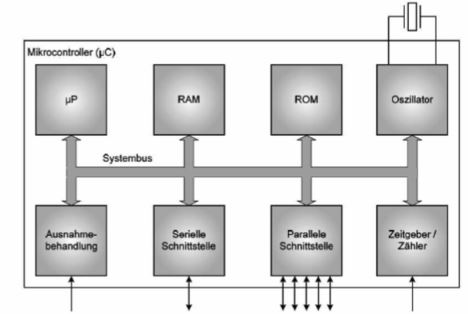
\includegraphics[width=\linewidth]{images/aufbauuC}
\end{minipage}

\begin{multicols}{2}
\subsubsection{Anwendungen}
\begin{minipage}{\linewidth}
\begin{itemize}
    \item Supercomputer
    \item Arbeits und Server-Rechnern
    \item Smartphones
    \item Navigationssysteme
    \item Digitalkameras
    \item Drucker
    \item ... TEst
\end{itemize}
\end{minipage}

\begin{minipage}{\linewidth}
\subsubsection{Aufbau von uP-basierten Systemen}
\begin{itemize}
    \item Zentraleinheit CPU mit
    \begin{itemize}
        \item Rechenwerk ALU
        \item Steuerwerk CU
        \item Registersatz
    \end{itemize}
    \item Speicher
    \item Eingabe-/Ausgabe-Schnittsellen
\end{itemize}
\end{minipage}
\end{multicols}

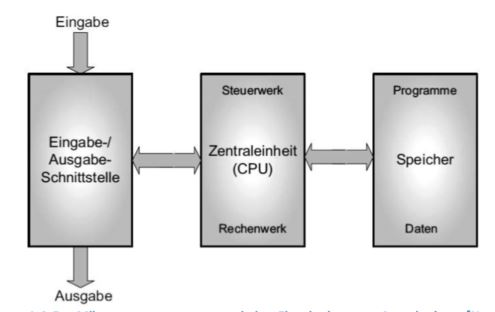
\includegraphics[width=0.5\linewidth]{images/aufbauuC1}
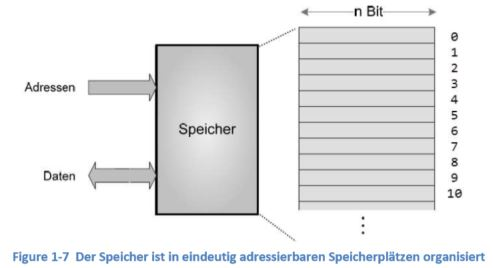
\includegraphics[width=0.5\linewidth]{images/aufbauuCspeicher}

\subsubsection{Havard vs Von Neumann Architektur}
\begin{multicols}{2}
    \begin{minipage}{\linewidth}
        \textbf{Harvard Rechnermodell}\\
        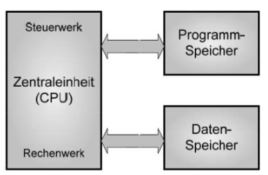
\includegraphics[width=0.6\linewidth]{images/HavardArchi}
    \end{minipage}
    
    \begin{minipage}{\linewidth}
        \textbf{von Neumann Rechnermodell}\\
        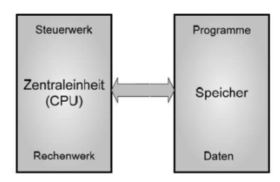
\includegraphics[width=0.6\linewidth]{images/NeumannArchi}
    \end{minipage}
\end{multicols}
\clearpage
%===================================
\subsubsection{Programmierung eins uP}
\begin{multicols}{2}
\begin{minipage}{\linewidth}
    Ein \mu P kann durch individuelle Programmierung auf ganz unterschiedliche Art angepasst werden. \newline
    \rightarrow entscheidend für die Durchdringung im Markt.\newline
    Ein Programm enthält in aufeinanderfolgender Anordnung die Maschinen-Befehle oder -Instruktionen für den \mu P. Diese Maschiene-Befehle teilen der CPU mit, welche Operationen in welcher Reihenfolge und auf welche Daten angewendet werden sollen. \newline
    Die Befehlsfolge des Programms wird innerhalb der CPU vom Steuerwerk gesteuert und schrittweise ausgeführt. Dazu wird der aktuell zur bearbeitende Befehl durch einen Programmzähler (PC) im Speicher adressiert.\newline
    Der PC enthält laufend die Adresse der Speicherzelle des jeweiligen Befehls im Speicher.
\end{minipage}

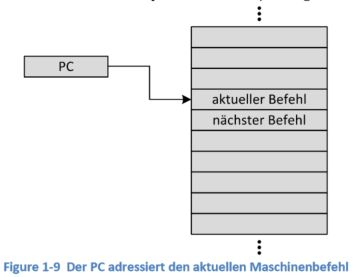
\includegraphics[width=\linewidth]{images/uPPC}
\end{multicols}
    
\subsubsection{Befehlsformate}
\begin{multicols}{2}
\begin{minipage}{\linewidth}
Die Art und Wirkung eines Befehls wird im Befehlswort (\textbf{OpCode}) codiert.
Darin sind neben der Operation auch die Operanden spezifiziert.
Die Codierung des Befehlswortes erfolgt abhängig vom \mu P.
Der Maschinencode setzt sich aus einem OpCode und einem oder mehreren Operanden zusammen.
\end{minipage}

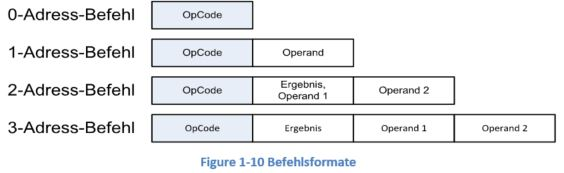
\includegraphics[width=\linewidth]{images/Befehlsformate}
\end{multicols}


\subsection{RISC vs CISC}
\begin{multicols}{2}
    \textbf{CISC}\newline
    Complex Instruction Set Computer
    \\
    \textbf{RISC}\newline
    Reduced Instruction Set Computer
\end{multicols}
\subsubsection{RISC-Rechner}
effizienter als CISC-Rechner
\begin{itemize}
    \item besteht aus einer kleinen Anz. von Befehlen mit wenigen Adressierungsarten
    \item Registersatz enthält eine grosse Anzahl von allg. verwendbaren Registern\newline
    General Purpose Register (GPR)
    \item Speicherzugriff erfolgt über spezielle Lade- und Speicher-Befehle
    \begin{itemize}
        \item Arithmetisch-logische Operationen arbeiten auf Registeroperanden
    \end{itemize}
    \item Pipeline-Architecture \leftarrow Leistungssteigernde Architektur
    \item Eine grosse semantische Lücke entsteht bei der Übersetzung aus der Hochsprache
\end{itemize}

\subsubsection{u Architektur}
Beschreibt die architektonischen Details bei der Implementierung der \mu P aus Sicht der Programmierer.
Dies umfasst die Beschreibung der Zentraleinheit (CPU), des Rechenwerks (ALU) und des Steuerwerks (CU).


\clearpage
\begin{minipage}{10cm}
\subsection{Hardware}
\subsubsection{Registersatz}
Register sind schnelle Zwischenspeicher für \newline
temporäre Daten im \mu P.
\end{minipage}
\begin{minipage}{0.5\linewidth}
\subsubsection{Hardware- /Software-Schnitsttelle}
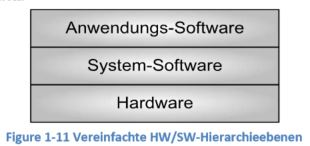
\includegraphics{images/HardwareSoftware}
\end{minipage}

\subsubsection{Taktfrequenz}
Das Taktsignal steuert die zeitliche Abfolge im \mu P \newline
\begin{multicols}{2}
        \begin{minipage}{\linewidth}
    \[ f_{Takt}= \frac{1}{T_{takt}} \]
        \end{minipage}
    
    \begin{minipage}{\linewidth}
        $ \Uparrow $ Taktrate $ \Leftrightarrow $$  \Uparrow  $Leistungsaufnahme \\
        Um Energie zu sparen ist es sinnvoll die Taktrate laufend anzupassen.\\
    \end{minipage}
\end{multicols}
\subsubsection{Leistungsaufnahme}
\begin{multicols}{2}
        \begin{minipage}{\linewidth}
\[ P_{Gate}= \frac{1}{2} \cdot C_{Last} \cdot V_{DD}^2\cdot f_{Takt} \]
    \end{minipage}
    
\begin{minipage}{\linewidth}
    $ P_{Gate} \qquad $Leistung pro CMOS Gate \newline
    $ C_{Last} \qquad $Lastkapazität\newline
    $ V_{DD}   \qquad $Versorgungsspannung\newline
    $ f_{Takt} \qquad $Taktfrequenz
\end{minipage}
\end{multicols}

\subsection{Software}
\begin{multicols}{2}
\subsubsection{Ablauf}
\begin{itemize}
    \item Der \textbf{Präprozessor} bereitet das Quellprogramm für den Compiler vor
    \item Der \textbf{Compiler} übersetzt das Programm von einer Hochsprache in ein Assembly-Programm
    \item Der \textbf{Binder} fasst verschiedene Dateien, die verschiebbaren Maschinencode enthalten, zu einem Programm zusammen.
    \item Der \textbf{Loader} wandelt die verschiebbaren Adressen in absolute Adressen um und lädt sie in den Speicher des Systems.
\end{itemize}

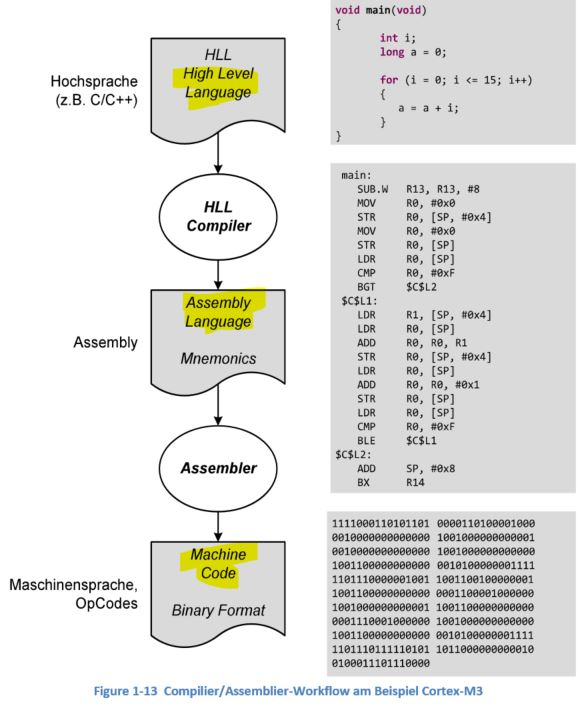
\includegraphics[width=\linewidth]{images/CompilerWorkflow}
\end{multicols}
\clearpage





















    